\documentclass[12pt,twoside]{article}

% packages
\usepackage{amssymb,amsmath,amsbsy}
\usepackage{graphicx}
\usepackage[includeheadfoot, top=1in, bottom=1in, hmargin=1in]{geometry}
\usepackage{fancyhdr}
\usepackage{verbatim}
\usepackage{url}
\usepackage{enumitem}
\usepackage{multicol}

% commands
\newcommand{\given}{\,|\,}
\newcommand{\dd}{\mathrm{d}}
\newcommand{\msun}{\mathrm{M}_\odot}
\newcommand{\projectname}[1]{\begin{center} {\huge {#1}} \end{center}}

% environments
\newcommand{\problemname}{Problem}
\newcounter{problem}
\newenvironment{problem}{\paragraph{\problemname~\theproblem:}\refstepcounter{problem}}{}
\newenvironment{problem0}{\paragraph{\problemname~0:}}{}
 
\pagestyle{fancy}

\lhead{Project 1}
\chead{}
\rhead{Adrian Price-Whelan}
\lfoot{Galactic Dynamics}
\cfoot{\thepage}
\rfoot{Fall 2014}

\begin{document}

\projectname{The Milky Way}

\begin{problem0}
To get started, 
	\begin{enumerate}
		\item install \texttt{Python} using the \texttt{Anaconda}\footnote{\url{https://store.continuum.io/cshop/anaconda}} distribution;
		\item update \texttt{Conda} and other packages by running:
			\begin{verbatim}
    % conda update conda
    % conda update numpy scipy astropy ipython
			\end{verbatim}
		\item verify that your installation worked by starting \texttt{IPython} and importing these packages:
			\begin{verbatim}
    % ipython
    In [1]: import numpy
    In [2]: import scipy.optimize
    In [3]: import astropy.coordinates
			\end{verbatim}
			you should not see any errors;
		\item download the Hipparcos data file.\footnote{\url{TODO: link to data}}
		
	\end{enumerate}
	
The data file contains kinematic information for 116,733 stars observed during the Hipparcos astrometric mission. The columns in the data file are:
\begin{multicols}{2}
	\begin{enumerate}[align=left,leftmargin=!,label={\bf Col. \arabic*:}]
		\item Hipparcos ID
		\item Galactic longitude, $l$ (degree)
		\item Galactic latitude, $b$ (degree)
		\item Parallax, $\pi$ (mas)
		\item Proper motion in $l$, $\mu_l$ (mas~yr$^{-1}$)
		\item Proper motion in $b$, $\mu_b$ (mas~yr$^{-1}$)
		\item Uncertainty in $\pi$, $\sigma_\pi$ (mas)
		\item Uncertainty in $\mu_l$, $\sigma_{\mu_l}$ (mas)
		\item Uncertainty in $\mu_b$, $\sigma_{\mu_b}$ (mas)
		\item $V$ magnitude
		\item $B-V$ color
		\item Multiplicity flag (you want this to be 0)
	\end{enumerate}
\end{multicols}
\end{problem0}

\begin{problem}
The goal is to read in the data file and generate a Hertzsprung-Russell diagram from the data. You'll need to use the parallax to get a distance to each star, then convert the apparent $V$-band magnitude into an absolute magnitude. You will want to select a sub-sample of stars that have good parallax measurements (e.g., $\sigma_\pi / \pi \lesssim 10\%$ or whatever you want) so that the distance conversions make sense. Even with this cut, you might end up with some strange outliers -- check that there are no crazy distance outliers.

You will also want to remove binary and multiple star systems from your sample. Do this by requiring that the multiplicity field is 0.

Make a plot of the $B-V$ color vs. absolute $V$-band magnitude for all stars remaining in your sample. Set the $x$-axis limits to $(-0.5,2.)$ and the $y$-axis limits to $(15,-5)$ -- note the inversion. Do you notice anything strange about the distribution of points in this plot? Extra credit if you make a \emph{density} plot instead of a scatter plot by making a 2D histogram of the data (e.g., right panel of figure below).

{\bf (10 pts)}

\begin{figure}[!h]
\begin{center}
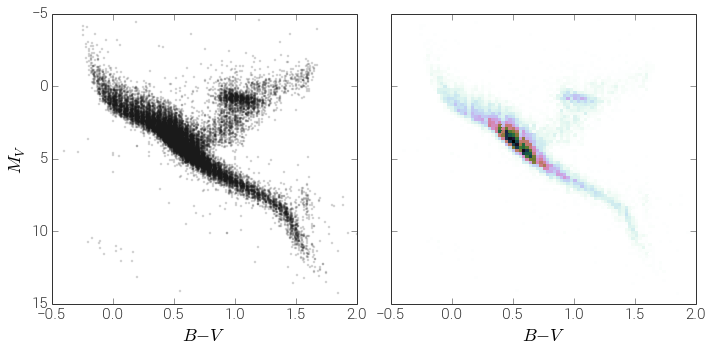
\includegraphics[width=\textwidth]{hr-diag.png}
\caption{ H-R diagram of Hipparcos stars. }\label{fig:hrdiag}
\end{center}
\end{figure}

\end{problem}

\begin{problem}
Estimate Oort constants from Hipparcos proper motions
\end{problem}

\begin{problem}
Repeat for MS / evolved, compare and why
\end{problem}

\end{document}

%\begin{figure*}[!h]
%\begin{center}
%\includegraphics[width=\textwidth]{PATH}
%\caption{ CAPTION }\label{fig:FIGNAME}
%\end{center}
%\end{figure*}